% Chapter Template

\chapter{Αξιολόγηση παραγόμενων κοινοτήτων} % Main chapter title

\label{Αξιολόγηση} % Change X to a consecutive number; for referencing this chapter elsewhere, use \ref{ChapterX}

\lhead{Κεφάλαιο 5. \emph{Αξιολόγηση παραγόμενων κοινοτήτων}} % Change X to a consecutive number; this is for the header on each page - perhaps a shortened title

\noindent
Εδώ περιγράφεται η προσέγγιση και οι μέθοδοι που αφορούν την αξιολόγηση των παραγόμενων κοινοτήτων (Εvaluation). 
Περιγράφονται σε ξεχωριστό κεφάλαιο αφού το Evaluation δεν αποτελεί λειτουργία του socialPServer αλλά εργαλείο του προγραμματιστή ώστε 
να μπορεί να συγκρίνει την απόδοση των αλγορίθμων.\\

Το πρόβλημα στην διαδικασίας αξιολόγησης είναι ότι δεν μπορεί να είναι ακριβής αν δεν υπάρξει ανάδραση από τους χρήστες. 
Αν δηλαδή δεν είναι γνωστό σε πιο βαθμό τα μέλη μιας κοινότητας έχουν όντως κοινά ενδιαφέροντα και προτιμήσεις.
Για να ξεπεραστεί αυτό το πρόβλημα και να υπάρχουν στοιχεία αξιολόγησης, υλοποιήθηκαν οι παρακάτω μέθοδοι στις οποίες,
έχοντας ένα DataSet που περιέχει ρεαλιστική κοινωνική πληροφορία μεταξύ των χρηστών αλλά και τις προτιμήσεις αυτών, ελέγχεται σε πιο βαθμό
υπάρχει \emph{ομοιότητα} στις αξιολογήσεις των αντικειμένων στα πλαίσια της κάθε κοινότητας.
Καθώς επίσης και σε ποιο βαθμό υπάρχει \emph{ανομοιότητα} στις αξιολογήσεις μεταξύ των διαφορετικών κοινοτήτων. 
Πρόκειται επομένως για \textbf{Εσωτερική Αξιολόγηση}.
Ακολουθεί πιο αναλυτική περιγραφή της μεθόδου καθώς και παρουσίαση των DataSet που χρησιμοποιήθηκαν.


\section{Δεδομένα (DataSets)}
\noindent
Όπως προαναφέρθηκε για να γίνει αξιολόγηση πρέπει να υπάρχουν πληροφορίες τόσο για την κοινωνική σχέση των χρηστών αλλά και για τις προτιμήσεις τους σε αντικείμενα.
Για να είναι ρεαλιστική και να έχει αποτέλεσμα η διαδικασία δεν αρκεί να δημιουργηθεί ένα ενδεικτικό σύνολο δεδομένων παράγοντας τυχαίες συνδέσεις φιλίας
και τυχαίες αξιολογήσεις αντικειμένων γιατί έτσι χάνεται το όλο νόημα της \emph{κοινωνικής πληροφορίας} η οποία εμπεριέχεται σε πραγματικούς κοινωνικούς γράφους.

Επομένως πρέπει να χρησιμοποιηθούν ρεαλιστικά δεδομένα.
Τέτοιου είδους δεδομένα σπανίζουν και συνήθως πληρώνονται αδρά, για αυτό και παρατηρείται η μανιωδώς 
συλλογή προσωπικών δεδομένων των χρηστών από τις μεγάλες εμπορικές πλατφόρμες που εμπεριέχουν κοινωνική δικτύωση.

Υπάρχουν όμως κάποια DataSets που είναι ανοιχτά για το κοινό, βοηθώντας την έρευνα, 
στα οποία είναι βασισμένες οι περισσότερες δημοσιεύσεις στον συγκεκριμένο τομέα.
Στην παρούσα εργασία εντοπίσαμε τα ακόλουθα σύνολα δεδομένων:

\begin{description}
\item \textbf{Last.FM Dataset}  \hfill \\
Πρόκειται για ένα σύνολο δεδομένων που έχει εξαχθεί χρησιμοποιώντας την υπηρεσία μουσικής προσωποποίησης Last FM\cite{LastFM} το οποίο παρουσιάστηκε κατά τη διάρκεια του 
 \setlanguage{english} 
\emph{2nd International Workshop on Information Heterogeneity and Fusion in Recommender Systems στο 5th ACM Conference on Recommender Systems}\cite{RecSys2011}.\\
 \setlanguage{greek}
Περιλαμβάνει κοινωνική δικτύωση και αξιολογήσεις καλλιτεχνών, στοιχεία που το καθιστούν ιδανικό για την δικιά μας περίπτωση.
Η έκδοση που χρησιμοποιήσαμε αποτελείται από 1892 χρήστες με 12717 ακμές φιλίας δηλαδή 25434 εγγραφές του τύπου: $undirected (user_i, user_j)$, 
όπου ο κάθε χρήστης έχει 13,443 φίλους κατά μέσο όρο.
Επίσης δίνονται 92834 αξιολογήσεις καλλιτεχνών (αντικείμενα).\\
Η συγκεκριμένη έκδοση είναι δανεισμένη από το \emph{Grouplens}\cite{grouplens}.\\
Πρόκειται για \emph{Undirected Graph}.
\item \textbf{Flixster Dataset}  \hfill \\
Δεδομένα από το Flixster.com\cite{flixster}, μια πλατφόρμα για εύρεσης ταινιών. Προσφέρει την δυνατότητα αξιολόγησης ταινιών και μπορεί να εγκατασταθεί σε κοινωνικά δίκτυα
από όπου και αντλήθηκε η πληροφορία φιλίας. Επομένως δίνει social και rating πληροφορία. 
Η έκδοση που χρησιμοποιήσαμε είναι αυτή του Mohsen Jamali\cite{MohsenJamali} η οποία περιλαμβάνει 7058820 εγγραφές φιλίας του τύπου: $undirected (user_i, user_j)$ και
8196078 αξιολογήσεις τενιών (ανικημένων).\\
Πρόκειται για \emph{Undirected Graph}.
\item \textbf{Epinions Dataset}  \hfill \\
Πρόκειται για μία διαδικτυακή υπηρεσία αξιολόγησης αντικειμένων, στην οποία κάποιος έχει την δυνατότητα να δηλώσει εμπιστοσύνη ή όχι για κάποιον άλλο χρήστη. 
Επομένως υπάρχει η πληροφορία trust-distrust η οποία συμβολίζεται με 1 ή -1 άλλα και τα ratings των αντικειμένων.\\
Αφού είναι trust και όχι social network πρόκειται για \emph{Directed Graph}. \cite{massa2006trust}
\end{description} 

Για την αξιολόγηση του socialPServer δοκιμάστηκαν δεδομένα του LastFM και του Flixster των οποίων η φύση ταιριάζει περισσότερο στην παρούσα εργασία.

\section{Σχεδιασμός της μεθόδου Αξιολόγησης}
\noindent
Μέσω της πραγματικής χρήση του προγράμματος, κάποιος θα μπορούσε να πάρει το απαραίτητο feedback για την απόδοση του συστήματος,
συλλέγοντας στατιστικά από την συμπεριφορά των χρηστών ανάλογα με τον κάθε αλγόριθμο.
Θα μπορούσε επίσης με ένα λειτουργικό σύστημα συστάσεων, να κάνει 
προτάσεις στους χρήστες και ελέγξει το τι πραγματικά είδαν.
Στο παρόν στάδιο όμως καθώς δεν έχει ολοκληρωθεί η λειτουργική ενσωμάτωση του socialPServer στον PServer, 
για να μπορεί να υπάρξει μιας μορφής αξιολόγηση και σύγκριση των αλγορίθμων 
  ακολουθείται η τυπική προσέγγιση εσωτερικής αξιολόγησης clustering που 
προτείνεται όταν στόχος είναι η ομοιότητα μεταξύ των χρηστών σε επίπεδο αντικειμένων.
Πιο συγκεκριμένα, η αξιολόγηση θεωρεί στόχο ενός "καλού" αλγορίθμου την εύρεση κοινοτήτων με 
\textbf{υψηλή intra-cluster similarity} (οι χρήστες μέσα σε μία κοινότητα είναι \emph{όμοιοι} σε επίπεδο αντικειμένων) και 
\textbf{χαμηλή inter-cluster similarity} (οι χρήστες που ανήκουν σε διαφορετικές κοινότητες είναι \emph{ανόμοιοι} σε επίπεδο αντικειμένων).
Πρόκειται για ένα κριτήριο \emph{εσωτερικής} αξιολόγησης και πρέπει να σημειωθεί πως καλή εσωτερική αξιολόγηση δεν σημαίνει απαραίτητα και καλή απόδοση του προγράμματος.\\
\cite{manning2008introduction}

Η υλοποίηση μας είναι βασισμένη στην μέθοδο αξιολόγησης \emph{Davies–Bouldin index} \cite{DaviesBouldinIndex}, η οποία παραλλάχθηκε ώστε να έχει νόημα
για την περίπτωση. 

Ποιο αναλυτικά, χρησιμοποιείται ένα μέτρο \textbf{ποιότητας συσταδοποίησης} για του οποίου τον υπολογισμό λαμβάνουν μέρος επιμέρους υπολογισμοί ομοιότητας 
(και όχι απόστασης όπως στην περίπτωση του Davies–Bouldin index).
Το μέτρο ποιότητας υπολογίζεται ως εξής:

$ Quality = \frac{Intra Simmilarity}{Inter Simmilarity}  $

όπου το Intra (Similarity) είναι η ομοιότητα που υπάρχει μεταξύ των μελών του ίδιου cluster και Inter (Similarity) η ομοιότητα που έχουν μεταξύ τους οι χρήστες διαφορετικών clusters.
Όπως είναι προφανές στόχος του κάθε αλγορίθμου είναι να έχει υψηλό Intra και χαμηλό Inter Simmilarity. 
Για αυτό και η ποιότητα υπολογίζεται με τον λόγο αυτών των δύο ώστε να τηρούνται οι
αναλογίες και να μπορούμε να συγκρίνουμε τους διαφορετικούς αλγορίθμους, με καλύτερο τον αλγόριθμο που έχει τον μεγαλύτερο λόγο (quality).
Ακολουθεί η ποιο αναλυτική περιγραφή για το πως υπολογίζονται τα μέτρα Intra και Inter Simmilarity αφού πρώτα αναφερθούμε σε κάποιες βασικές δομικές έννοιες.

\subsection{Αντιπροσωπευτικό σημείο συστάδας - centroid}
\noindent
Το πρόγραμμα μπορεί να εξυπηρετεί μεγάλο αριθμό χρηστών και τα αντικείμενα της υπηρεσίας μπορεί επίσης να είναι πάρα πολλά επομένως, η σύγκριση όλων των προφίλ χρηστών
σε μία κοινότητα μεταξύ τους θα ήταν μια δαπανηρή διαδικασία τόσο σε επίπεδο χρόνου αλλά και πόρων. 
Για αυτό υπολογίζονται και χρησιμοποιούνται κεντροϊδή σε κάθε συστάδα \textbf{Centroids}.
Για κάθε cluster δημιουργείται ένα ακόμα φανταστικό μέλος του οποίο το προφίλ (αξιολογήσεις) είναι το μέσο των αξιολογήσεων όλων των άλλων μελών. 
Αυτός ο εικονικός κόμβος είναι ουσιαστικά το κέντρο βάρους του γράφου των αντικειμένων - το σημείο που βρίσκεται στο κέντρο των αποστάσεων των προφίλ των χρηστών.
Με αυτό τον τρόπο αντί να υπολογίζεται η ομοιότητα όλων των προφίλ των χρηστών μεταξύ τους υπολογίζεται η ομοιότητα του κάθε χρήστη με τον εικονικό χρήστη Centroid.

\subsection{Μετρική ομοιότητας - cosine similarity}
\noindent
Υπάρχουν πολλές μετρικές που θα μπορούσαν να χρησιμοποιηθούν και να εκφράσουν την ομοιότητα δύο προφίλ χρηστών. 
Μία από τις πιο διαδεδομένες την οποία επιλέξαμε να χρησιμοποιήσουμε είναι η \textbf{Cosine similarity}. 
Η ομοιότητα Cosine συγκεκριμένα μετράει το συνημίτονο (cos) της γωνίας μεταξύ των δύο προφίλ.
Από την φύση της παίρνει τιμές από -1 εώς 1 αλλά στις περιπτώσεις που οι αρνητικές τιμές δεν έχουν νόημα, όπως και εδώ, παίρνει τιμές από 0 ως 1.

Ο τύπος του υπολογισμού της:

$ cosineSimilarity(A,B) = \frac{A \cdot B}{\|A\|\|B\|} = \frac{\sum\limits_{i=1}^n A_i \times B_i}{\sqrt{\sum\limits_{i=1}^n (A_i)^2} \times \sqrt{\sum\limits_{i=1}^n (B_i)^2}} $

\subsection{Μετρική ομοιότητας ζεύγους συστάδων - Intra Simmilarity}
\noindent
Ομοιότητα των μελών που βρίσκονται στο ίδιο cluster:

Έστω
\begin{description}
\item \textbf{C} το πλήθος των clusters  
\item \textbf{M} το πλήθος όλων των μελών όλων των cluster
\item \textbf{m} το πλήθος των μελών του κάθε cluster
\item \textbf{x} το κάθε Cluster
\end{description} 

βασικές έννοιες:
\begin{description}
\item \textbf{ratio(x)} cluster x size Ratio: βάρος του κάθε cluster στο συνολικό αποτέλεσμα
\item \textbf{comp(x)} cluster x Compuctness: εσωτερική ομοιότητα του κάθε cluster
\end{description} 


$ Intra = \sum\limits_{x=1}^C  comp(x) * ratio(x) $

$ ratio(x) = \frac{m_x}{M} $

\begin{description}
\item \textbf{cos(i,j)} cosine Simmilarity of memebers i - j 
\item \textbf{cent(x)} centroid of cluster x
\end{description} 


$ comp(x) = \frac{1}{m_x} * \sum\limits_{i=1}^{m_x} cos(i,cent(x)) $

Για τον υπολογισμό του \emph{Intra simmilarity} αθροίζουμε την εσωτερική ομοιότητα του κάθε cluster
πολλαπλασιασμένη με το \emph{Ratio} ώστε να επηρεάσει το τελικό αποτέλεσμα ανάλογα με το μέγεθός του.
Για να βρούμε την εσωτερική ομοιότητα του κάθε cluster (\emph{Compuctness}) αθροίζουμε την \emph{cosine simmilarity} 
του κάθε μέλους με το centroid του cluster. 

Επομένως προκύπτει:

$ InterSimmilarity = \frac{1}{M} \sum\limits_{x=1}^C \sum\limits_{i=1}^{m_x} cos(i,cent(x)) $

\subsection{Inter Simmilarity}
\noindent
Ομοιότητα των μελών που \textbf{δεν} βρίσκονται στο ίδιο cluster:

Με την ίδια λογική και σε αυτήν την περίπτωση αντί να συγκρίνουμε όλα τα μέλη των διαφορετικών κοινοτήτων
μεταξύ τους, θα συγκρίνουμε τα \emph{centroids} όλων των κοινοτήτων. 

Επομένως:

$ Inter Simmilarity = \sum\limits_{i,j=0}^C cos(cent(i),cent(j)) $

\begin{figure}[htbp]
  %\begin{center}
  \hspace{-7.5em}  
    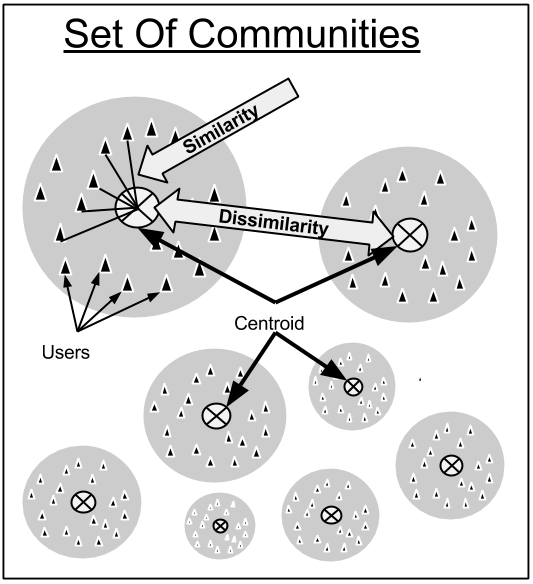
\includegraphics[scale=0.80]{Figures/evaluation_flow.png}
	\rule{35em}{0.5pt}  % UnderLine figure	
	\caption[evaluation_flow]{αξιολόγηση κοινοτήτων}
 %\end{center}	
  \label{fig:evaluation_flow}  
\end{figure}


%\vfill


\section{Υλοποίηση της Αξιολόγησης}
\label{eval}
\noindent
Οι μέθοδοι που σχετίζονται με την αξιολόγηση βρίσκονται κάθε φορά στην κλάση που αντιπροσωπεύει το αντικείμενο το οποίο θέλουμε να αξιολογήσουμε. 
Εφόσον αξιολογούνται αλγόριθμοι κάθε αλγόριθμος έχει μία μέθοδο \textbf{Evaluate}.\\
Ο κάθε αλγόριθμος περιέχει ένα αντικείμενο τύπου \textbf{SetOfCommunities} το 
οποίο αντιπροσωπεύει το σύνολο των παραγόμενων κοινοτήτων. Επομένως κάθε τέτοιου είδους αντικείμενο περιέχει επίσης μια μέθοδο \textbf{evaluation} την οποία καλεί ο εκάστοτε αλγόριθμος.
Η μέθοδος evaluation() του κάθε SetOfCommunities αναλαμβάνει να υπολογίσει το \textbf{Quality} του Set. 
Κατά την διαδικασία θα χρειαστεί να υπολογιστεί η εσωτερική ομοιότητα της κάθε κοινότητας. 
Και σε αυτήν την περίπτωση, κάθε αντικείμενο τύπου Community εμπεριέχει μια μέθοδο η οποία θα υπολογίσει το Intra Simmilarity της κάθε κοινότητας.


Κατά την διαδικασία της αξιολόγησης αρχικά υπολογίζονται κάποιες γενικές πληροφορίες για τις παραγόμενες κοινότητες όπως ο αριθμός των κοινοτήτων και το μέσο μέγεθος cluster 
και στην συνέχεια υπολογίζεται ο λόγος Quality που περιγράφτηκε παραπάνω.